% C3: Transform frequency heatmap (kernel x transform)
% Generated by scripts/generate_latex_figures.py
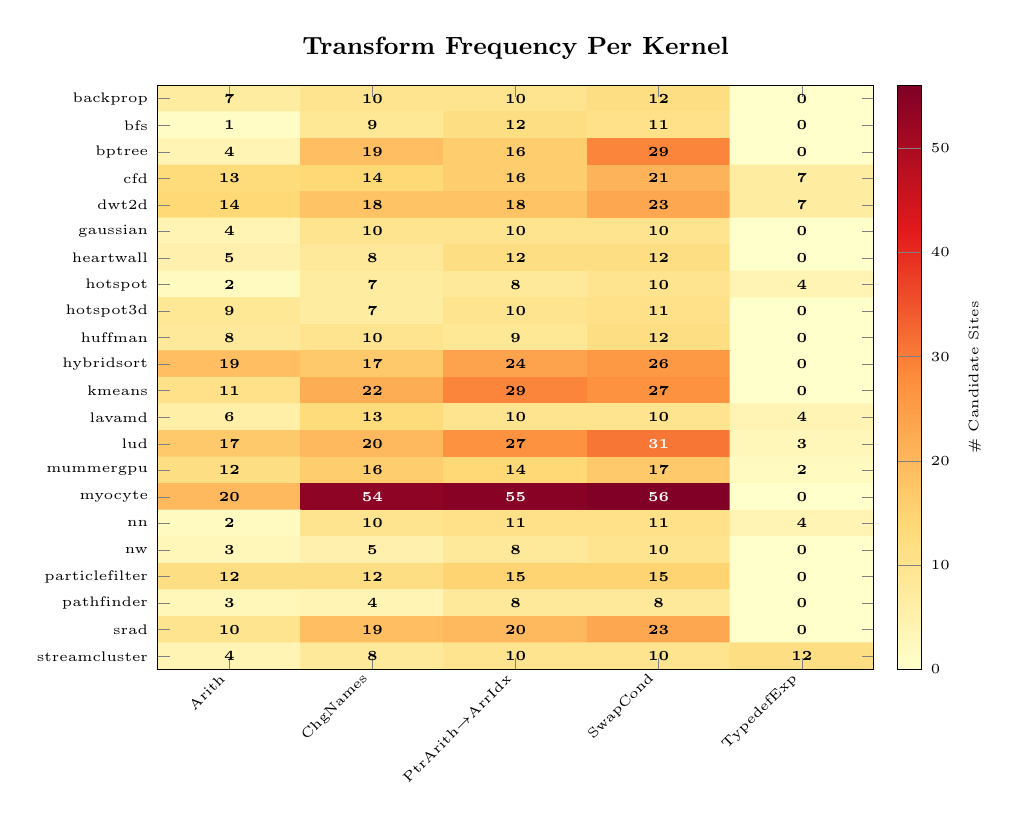
\begin{tikzpicture}
\begin{axis}[
  width=0.88\columnwidth,
  height=9cm,
  enlargelimits=false,
  axis on top,
  y dir=reverse,
  title style={font=\small\bfseries, align=center},
  tick label style={font=\tiny},
  colorbar,
  colorbar style={
    font=\tiny, width=0.3cm,
    ylabel={\# Candidate Sites},
    ylabel style={font=\tiny},
  },
  colormap={ylOrRd}{
    rgb255(0)=(255,255,204)
    rgb255(14)=(254,217,118)
    rgb255(28)=(253,141,60)
    rgb255(42)=(227,26,28)
    rgb255(56)=(128,0,38)
  },
  point meta min=0, point meta max=56,
  xtick={0,...,4},
  xticklabels={Arith,ChgNames,{PtrArith\ensuremath{\to}ArrIdx},SwapCond,TypedefExp},
  xticklabel style={font=\tiny, rotate=45, anchor=east},
  ytick={0,...,21},
  yticklabels={backprop,bfs,bptree,cfd,dwt2d,gaussian,heartwall,hotspot,hotspot3d,huffman,hybridsort,kmeans,lavamd,lud,mummergpu,myocyte,nn,nw,particlefilter,pathfinder,srad,streamcluster},
  yticklabel style={font=\tiny},
  xmin=-0.5, xmax=4.5,
  ymin=-0.5, ymax=21.5,
  title={Transform Frequency Per Kernel},
]
  %% Color matrix
  \addplot[matrix plot*, mesh/cols=5, point meta=explicit] coordinates {
    (0,0)[7]  (1,0)[10] (2,0)[10] (3,0)[12] (4,0)[0]
    (0,1)[1]  (1,1)[9]  (2,1)[12] (3,1)[11] (4,1)[0]
    (0,2)[4]  (1,2)[19] (2,2)[16] (3,2)[29] (4,2)[0]
    (0,3)[13] (1,3)[14] (2,3)[16] (3,3)[21] (4,3)[7]
    (0,4)[14] (1,4)[18] (2,4)[18] (3,4)[23] (4,4)[7]
    (0,5)[4]  (1,5)[10] (2,5)[10] (3,5)[10] (4,5)[0]
    (0,6)[5]  (1,6)[8]  (2,6)[12] (3,6)[12] (4,6)[0]
    (0,7)[2]  (1,7)[7]  (2,7)[8]  (3,7)[10] (4,7)[4]
    (0,8)[9]  (1,8)[7]  (2,8)[10] (3,8)[11] (4,8)[0]
    (0,9)[8]  (1,9)[10] (2,9)[9]  (3,9)[12] (4,9)[0]
    (0,10)[19] (1,10)[17] (2,10)[24] (3,10)[26] (4,10)[0]
    (0,11)[11] (1,11)[22] (2,11)[29] (3,11)[27] (4,11)[0]
    (0,12)[6]  (1,12)[13] (2,12)[10] (3,12)[10] (4,12)[4]
    (0,13)[17] (1,13)[20] (2,13)[27] (3,13)[31] (4,13)[3]
    (0,14)[12] (1,14)[16] (2,14)[14] (3,14)[17] (4,14)[2]
    (0,15)[20] (1,15)[54] (2,15)[55] (3,15)[56] (4,15)[0]
    (0,16)[2]  (1,16)[10] (2,16)[11] (3,16)[11] (4,16)[4]
    (0,17)[3]  (1,17)[5]  (2,17)[8]  (3,17)[10] (4,17)[0]
    (0,18)[12] (1,18)[12] (2,18)[15] (3,18)[15] (4,18)[0]
    (0,19)[3]  (1,19)[4]  (2,19)[8]  (3,19)[8]  (4,19)[0]
    (0,20)[10] (1,20)[19] (2,20)[20] (3,20)[23] (4,20)[0]
    (0,21)[4]  (1,21)[8]  (2,21)[10] (3,21)[10] (4,21)[12]
  };
  %% Black labels for light cells (value < 30)
  \addplot[
    only marks, mark=none, point meta=explicit,
    nodes near coords={\pgfmathfloattoint{\pgfplotspointmeta}\pgfmathresult},
    nodes near coords align={center},
    every node near coord/.style={font=\tiny\bfseries, text=black, inner sep=0pt}
  ] coordinates {
    (0,0)[7]  (1,0)[10] (2,0)[10] (3,0)[12] (4,0)[0]
    (0,1)[1]  (1,1)[9]  (2,1)[12] (3,1)[11] (4,1)[0]
    (0,2)[4]  (1,2)[19] (2,2)[16] (3,2)[29] (4,2)[0]
    (0,3)[13] (1,3)[14] (2,3)[16] (3,3)[21] (4,3)[7]
    (0,4)[14] (1,4)[18] (2,4)[18] (3,4)[23] (4,4)[7]
    (0,5)[4]  (1,5)[10] (2,5)[10] (3,5)[10] (4,5)[0]
    (0,6)[5]  (1,6)[8]  (2,6)[12] (3,6)[12] (4,6)[0]
    (0,7)[2]  (1,7)[7]  (2,7)[8]  (3,7)[10] (4,7)[4]
    (0,8)[9]  (1,8)[7]  (2,8)[10] (3,8)[11] (4,8)[0]
    (0,9)[8]  (1,9)[10] (2,9)[9]  (3,9)[12] (4,9)[0]
    (0,10)[19] (1,10)[17] (2,10)[24] (3,10)[26] (4,10)[0]
    (0,11)[11] (1,11)[22] (2,11)[29] (3,11)[27] (4,11)[0]
    (0,12)[6]  (1,12)[13] (2,12)[10] (3,12)[10] (4,12)[4]
    (0,13)[17] (1,13)[20] (2,13)[27]            (4,13)[3]
    (0,14)[12] (1,14)[16] (2,14)[14] (3,14)[17] (4,14)[2]
    (0,15)[20]                                   (4,15)[0]
    (0,16)[2]  (1,16)[10] (2,16)[11] (3,16)[11] (4,16)[4]
    (0,17)[3]  (1,17)[5]  (2,17)[8]  (3,17)[10] (4,17)[0]
    (0,18)[12] (1,18)[12] (2,18)[15] (3,18)[15] (4,18)[0]
    (0,19)[3]  (1,19)[4]  (2,19)[8]  (3,19)[8]  (4,19)[0]
    (0,20)[10] (1,20)[19] (2,20)[20] (3,20)[23] (4,20)[0]
    (0,21)[4]  (1,21)[8]  (2,21)[10] (3,21)[10] (4,21)[12]
  };
  %% White labels for dark cells (value >= 30)
  \addplot[
    only marks, mark=none, point meta=explicit,
    nodes near coords={\pgfmathfloattoint{\pgfplotspointmeta}\pgfmathresult},
    nodes near coords align={center},
    every node near coord/.style={font=\tiny\bfseries, text=white, inner sep=0pt}
  ] coordinates {
    (3,13)[31] (1,15)[54] (2,15)[55] (3,15)[56]
  };
\end{axis}
\end{tikzpicture}
